\documentclass[parskip=half]{scrartcl}
\usepackage[paperheight=8.25in, paperwidth=5.25in, textheight=7.25in, textwidth=4.25in, margin=0.5in]{geometry}

\usepackage{unicode-math}
\setmainfont{Tex Gyre Schola}
\setmathfont{Tex Gyre Schola Math}

\usepackage{eso-pic, graphicx}
\usepackage{tikz}

\usepackage{enumitem}
\usepackage{multicol} % Format list of playtesters in two columns

\usepackage{caption}
\usepackage{subcaption}
\renewcommand{\thesubfigure}{\arabic{subfigure}}

\setkomafont{section}{\setmainfont{Century Gothic-Bold}\Huge\color{blue}}
\setkomafont{subsection}{\setmainfont{Century Gothic-Bold}\huge\color{blue}}
\setkomafont{subsubsection}{\setmainfont{Century Gothic-Bold}\LARGE\color{blue}}


%% Adjust spacing before and after section headings
%\RedeclareSectionCommand[
%  runin=false,
%  beforeskip=1.0\baselineskip,
%  afterskip=-0.0\baselineskip
%]{section}
%
%% Adjust spacing before and after subsection headings
%\RedeclareSectionCommand[
%  runin=false,
%  beforeskip=1.0\baselineskip,
%  afterskip=-0.0\baselineskip
%]{subsection}
%
%% Adjust spacing before and after subsubsection headings
%\RedeclareSectionCommand[
%  runin=false,
%  beforeskip=1.0\baselineskip,
%  afterskip=-0.0\baselineskip
%]{subsubsection}
%

\color{black}
\raggedright
\begin{document}
\AddToShipoutPictureBG*{
\includegraphics[width=\paperwidth,height=\paperheight]{blue_page.jpg}}
\begin{center}

\includegraphics[width=\textwidth]{rebound_logo.png}

\vfill

\includegraphics[width=\textwidth]{rebound_board.png}
\end{center}
\bigskip
\LARGE
\phantom{a}\hfill\textcolor{white}{Designed by Michael Purcell}\hfill\phantom{a}

\newpage
\normalsize

\begin{figure}
\begin{subfigure}{0.45\textwidth}
\raggedright
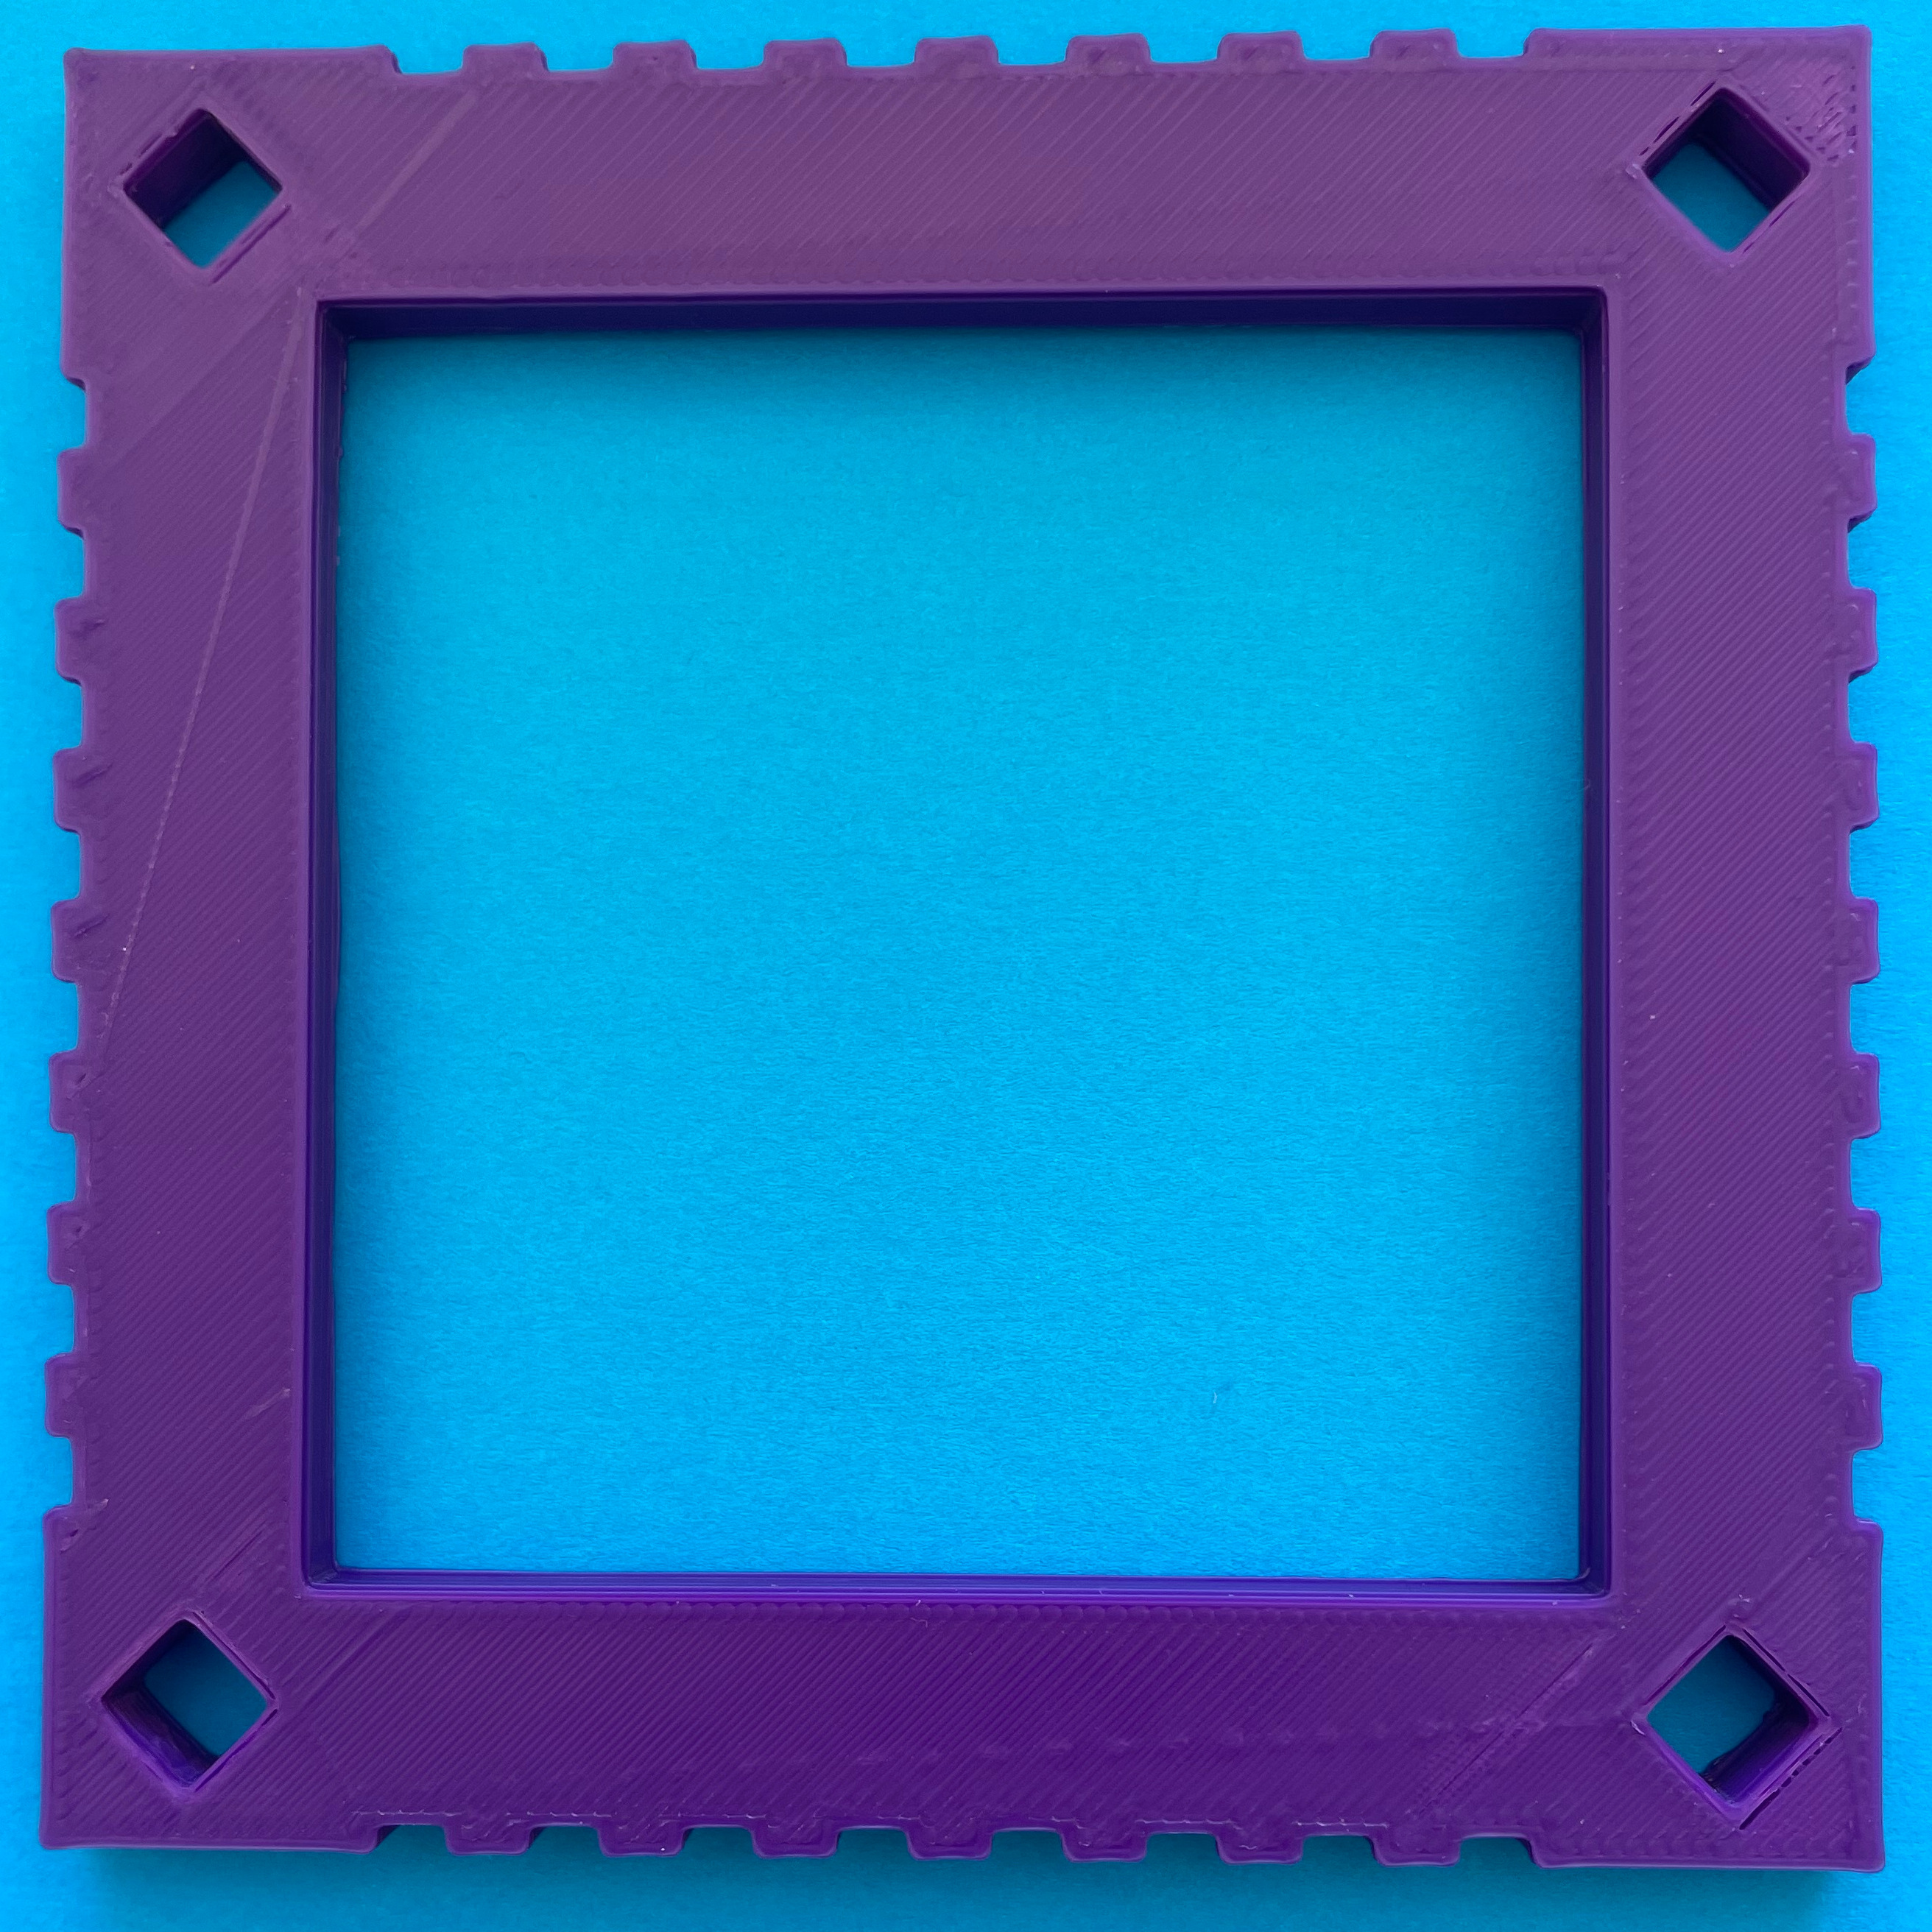
\includegraphics[width=\textwidth]{assembly_photo_1.jpg}
\caption{\raggedright \ Punch the trampoline}
frame and the trampoline feet out of the acrylic slug.
\end{subfigure}
\hfill
\begin{subfigure}{0.45\textwidth}
\raggedright
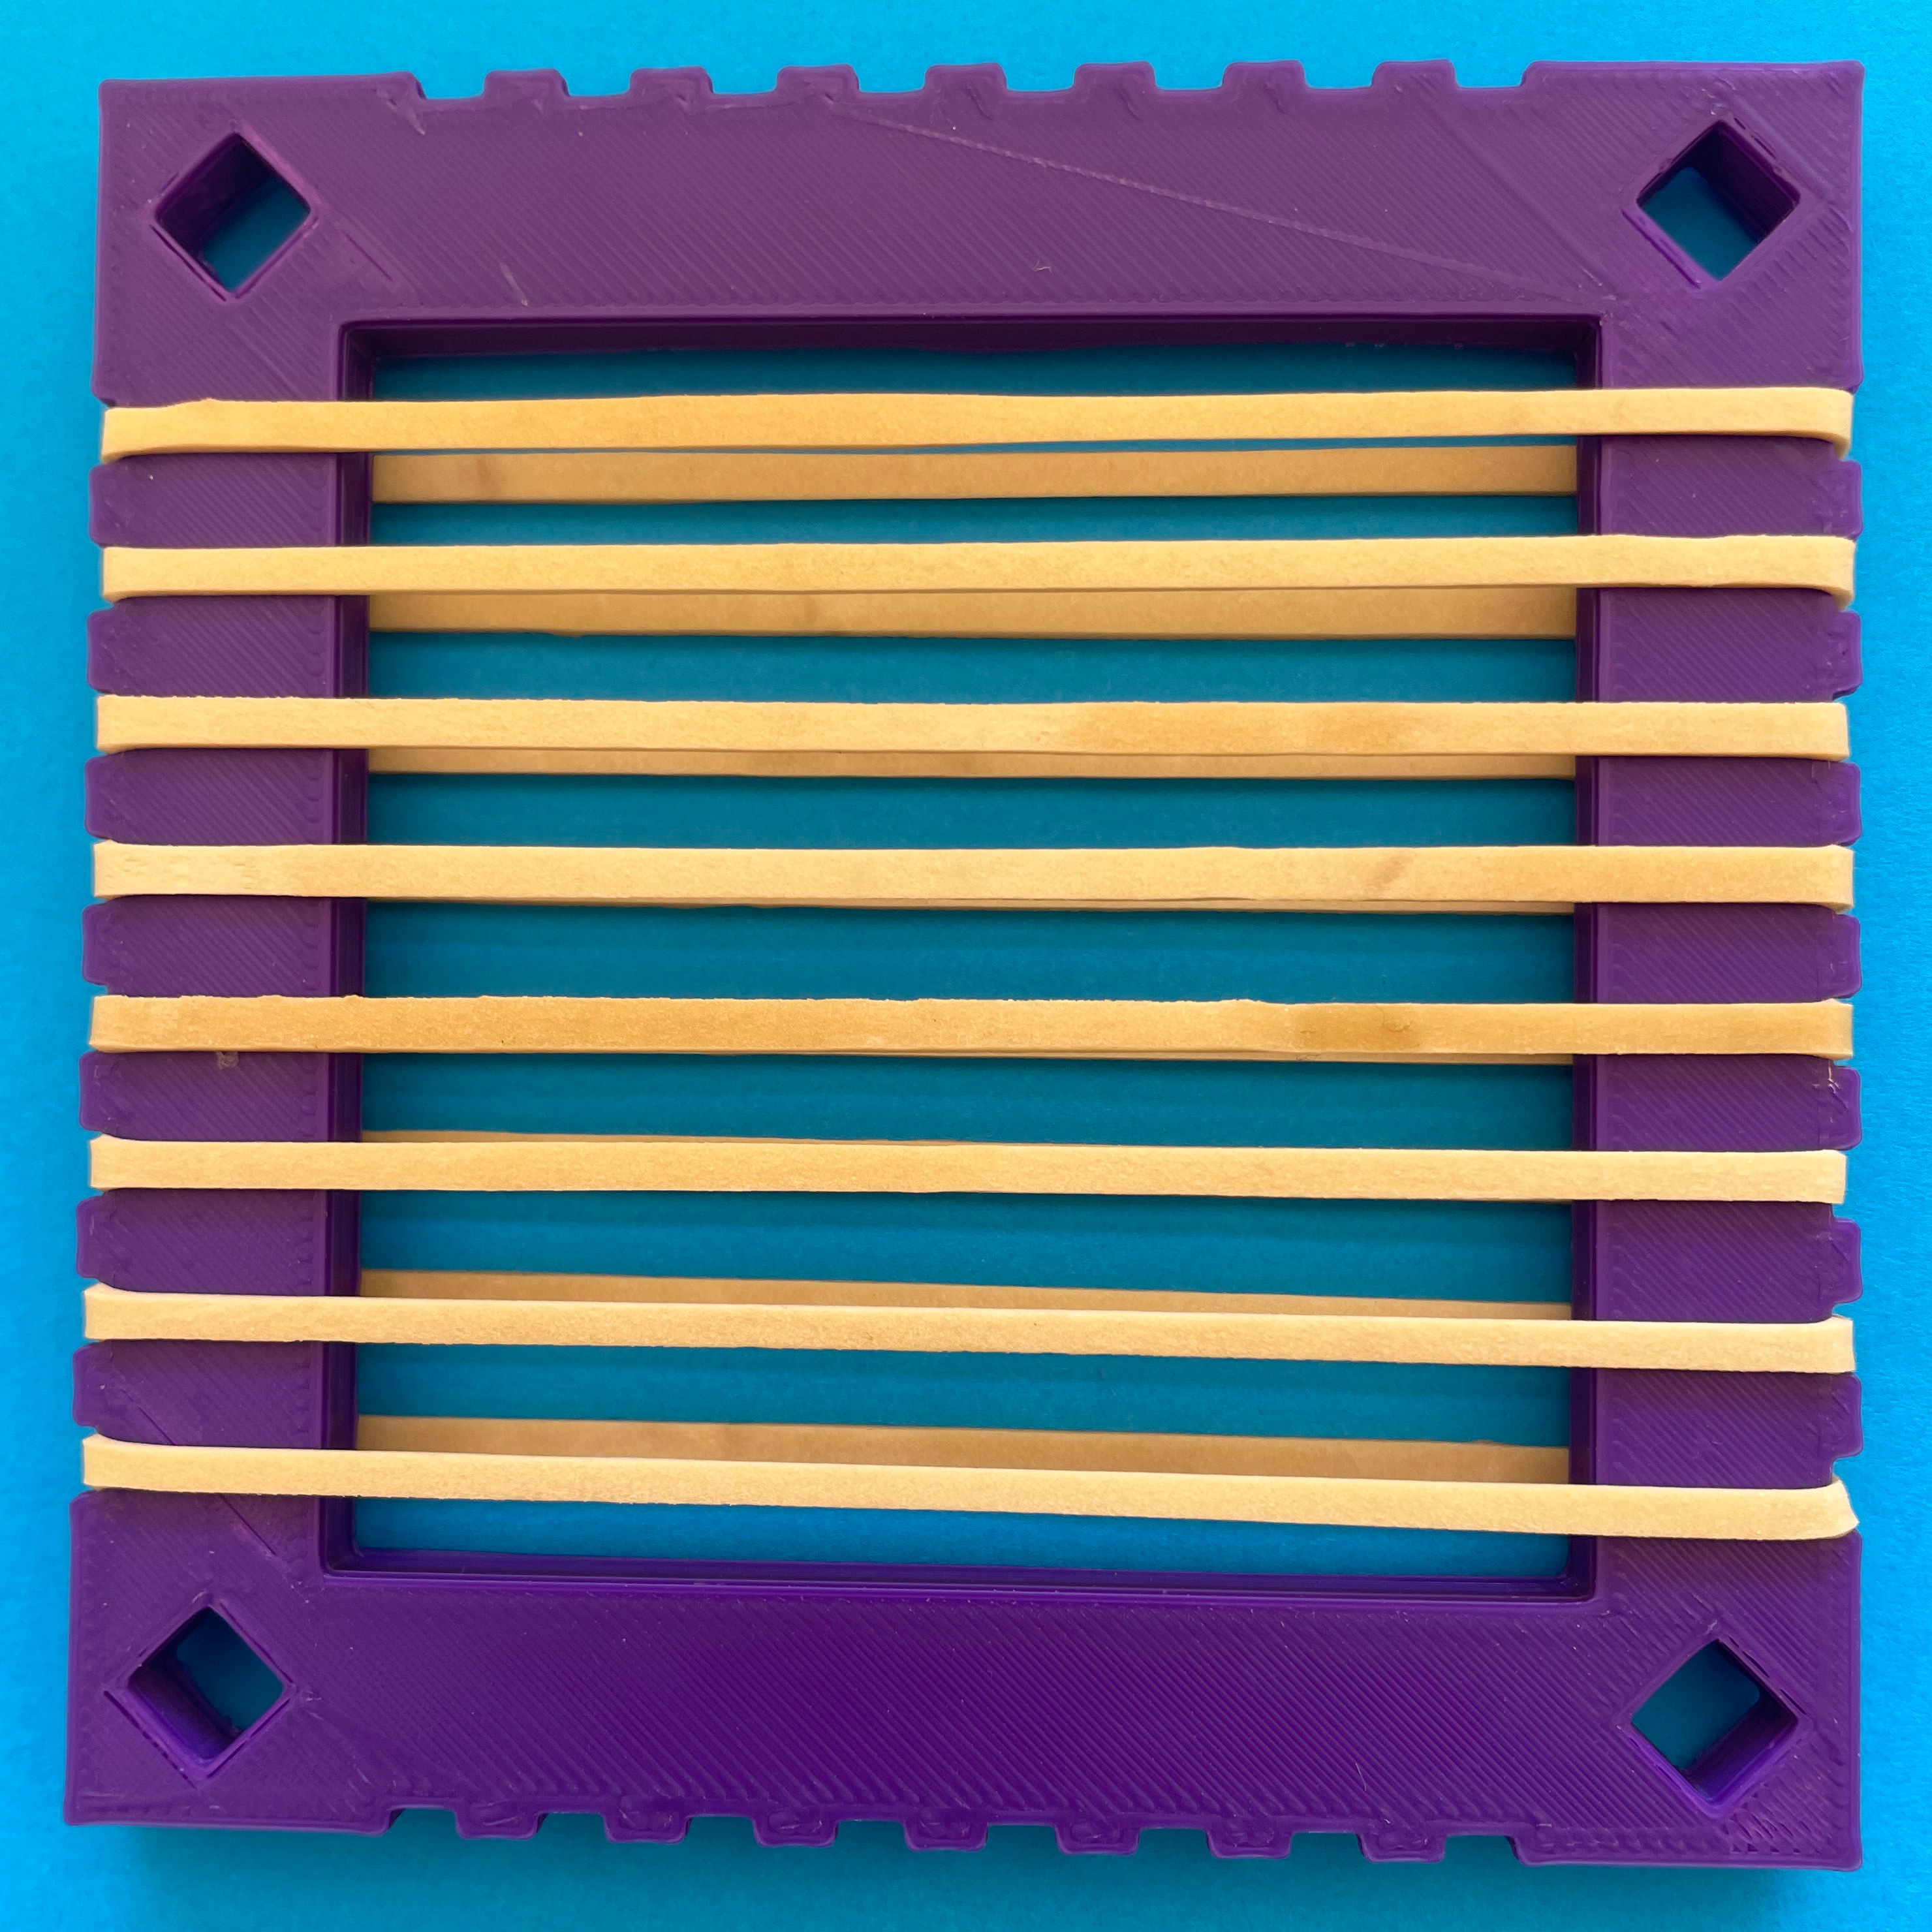
\includegraphics[width=\textwidth]{assembly_photo_2.jpg}
\caption{\raggedright \ Loop eight rubber bands}
horizontally around the trampoline frame.
\end{subfigure}

\vspace{0.1\textwidth}

\begin{subfigure}{0.45\textwidth}
\raggedright
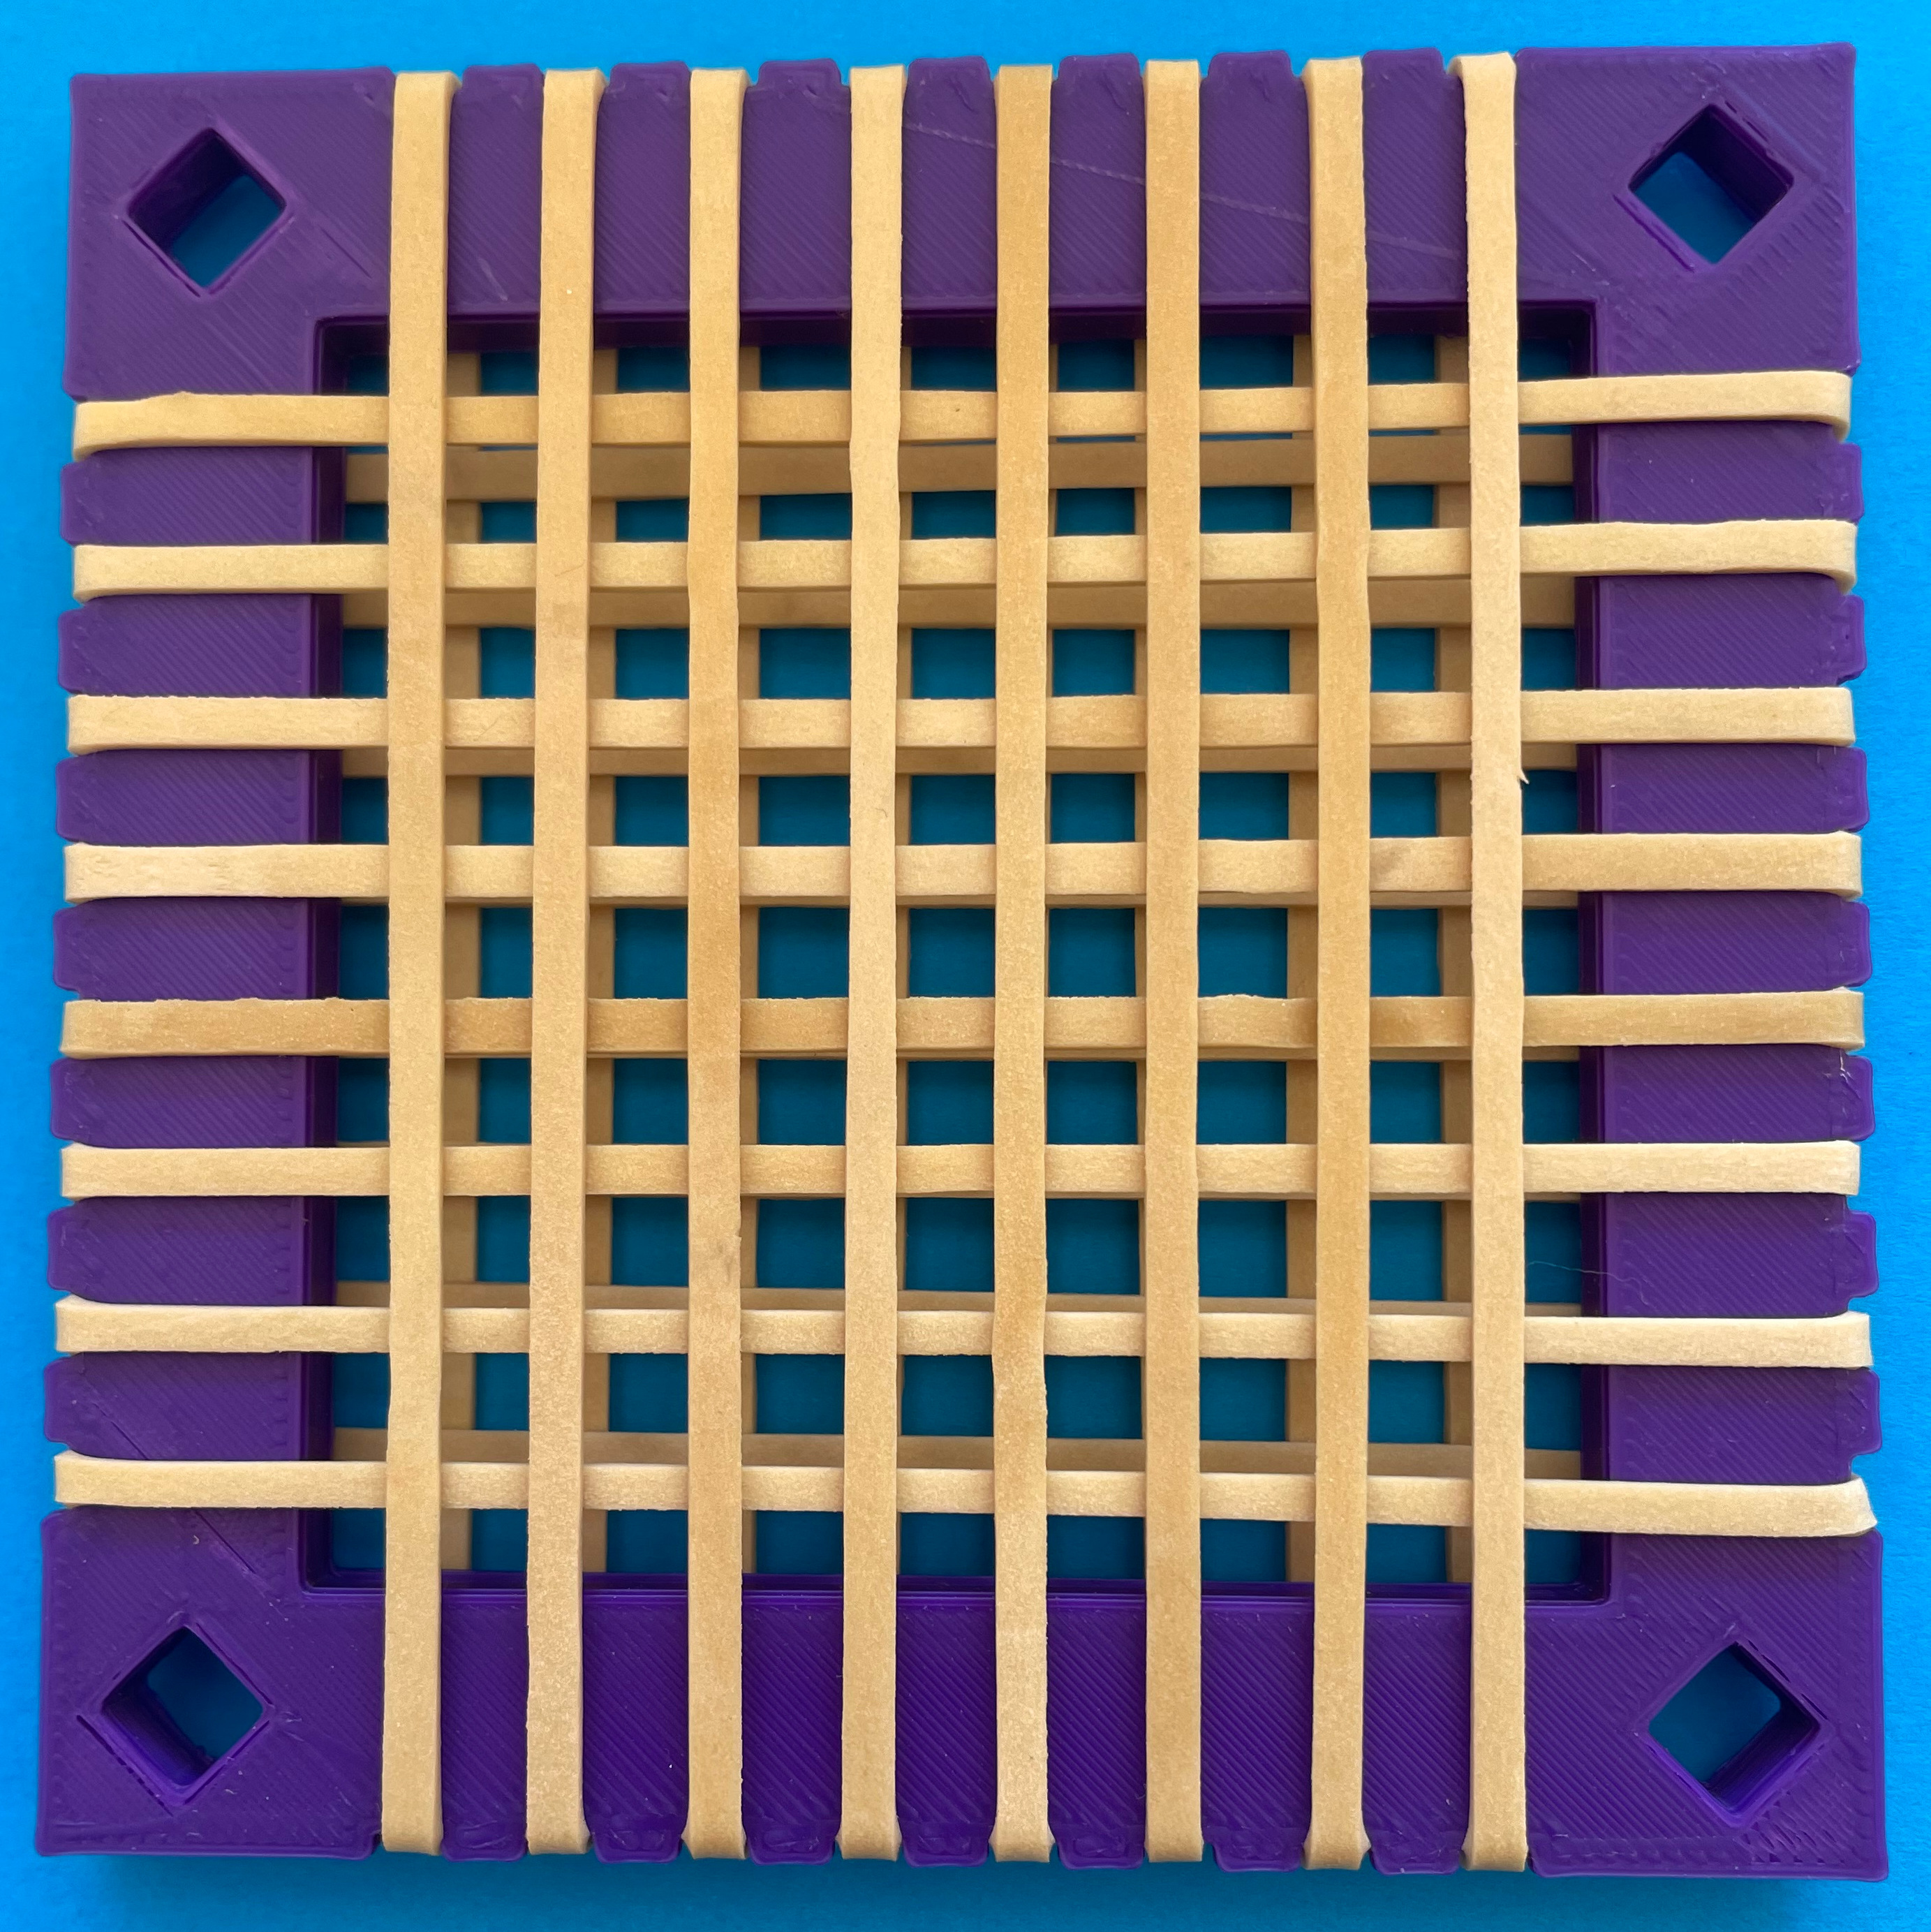
\includegraphics[width=\textwidth]{assembly_photo_3.jpg}
\caption{\raggedright \ Loop eight rubber bands}
vertically around the trampoline frame.
\end{subfigure}
\hfill
\begin{subfigure}{0.45\textwidth}
\raggedright
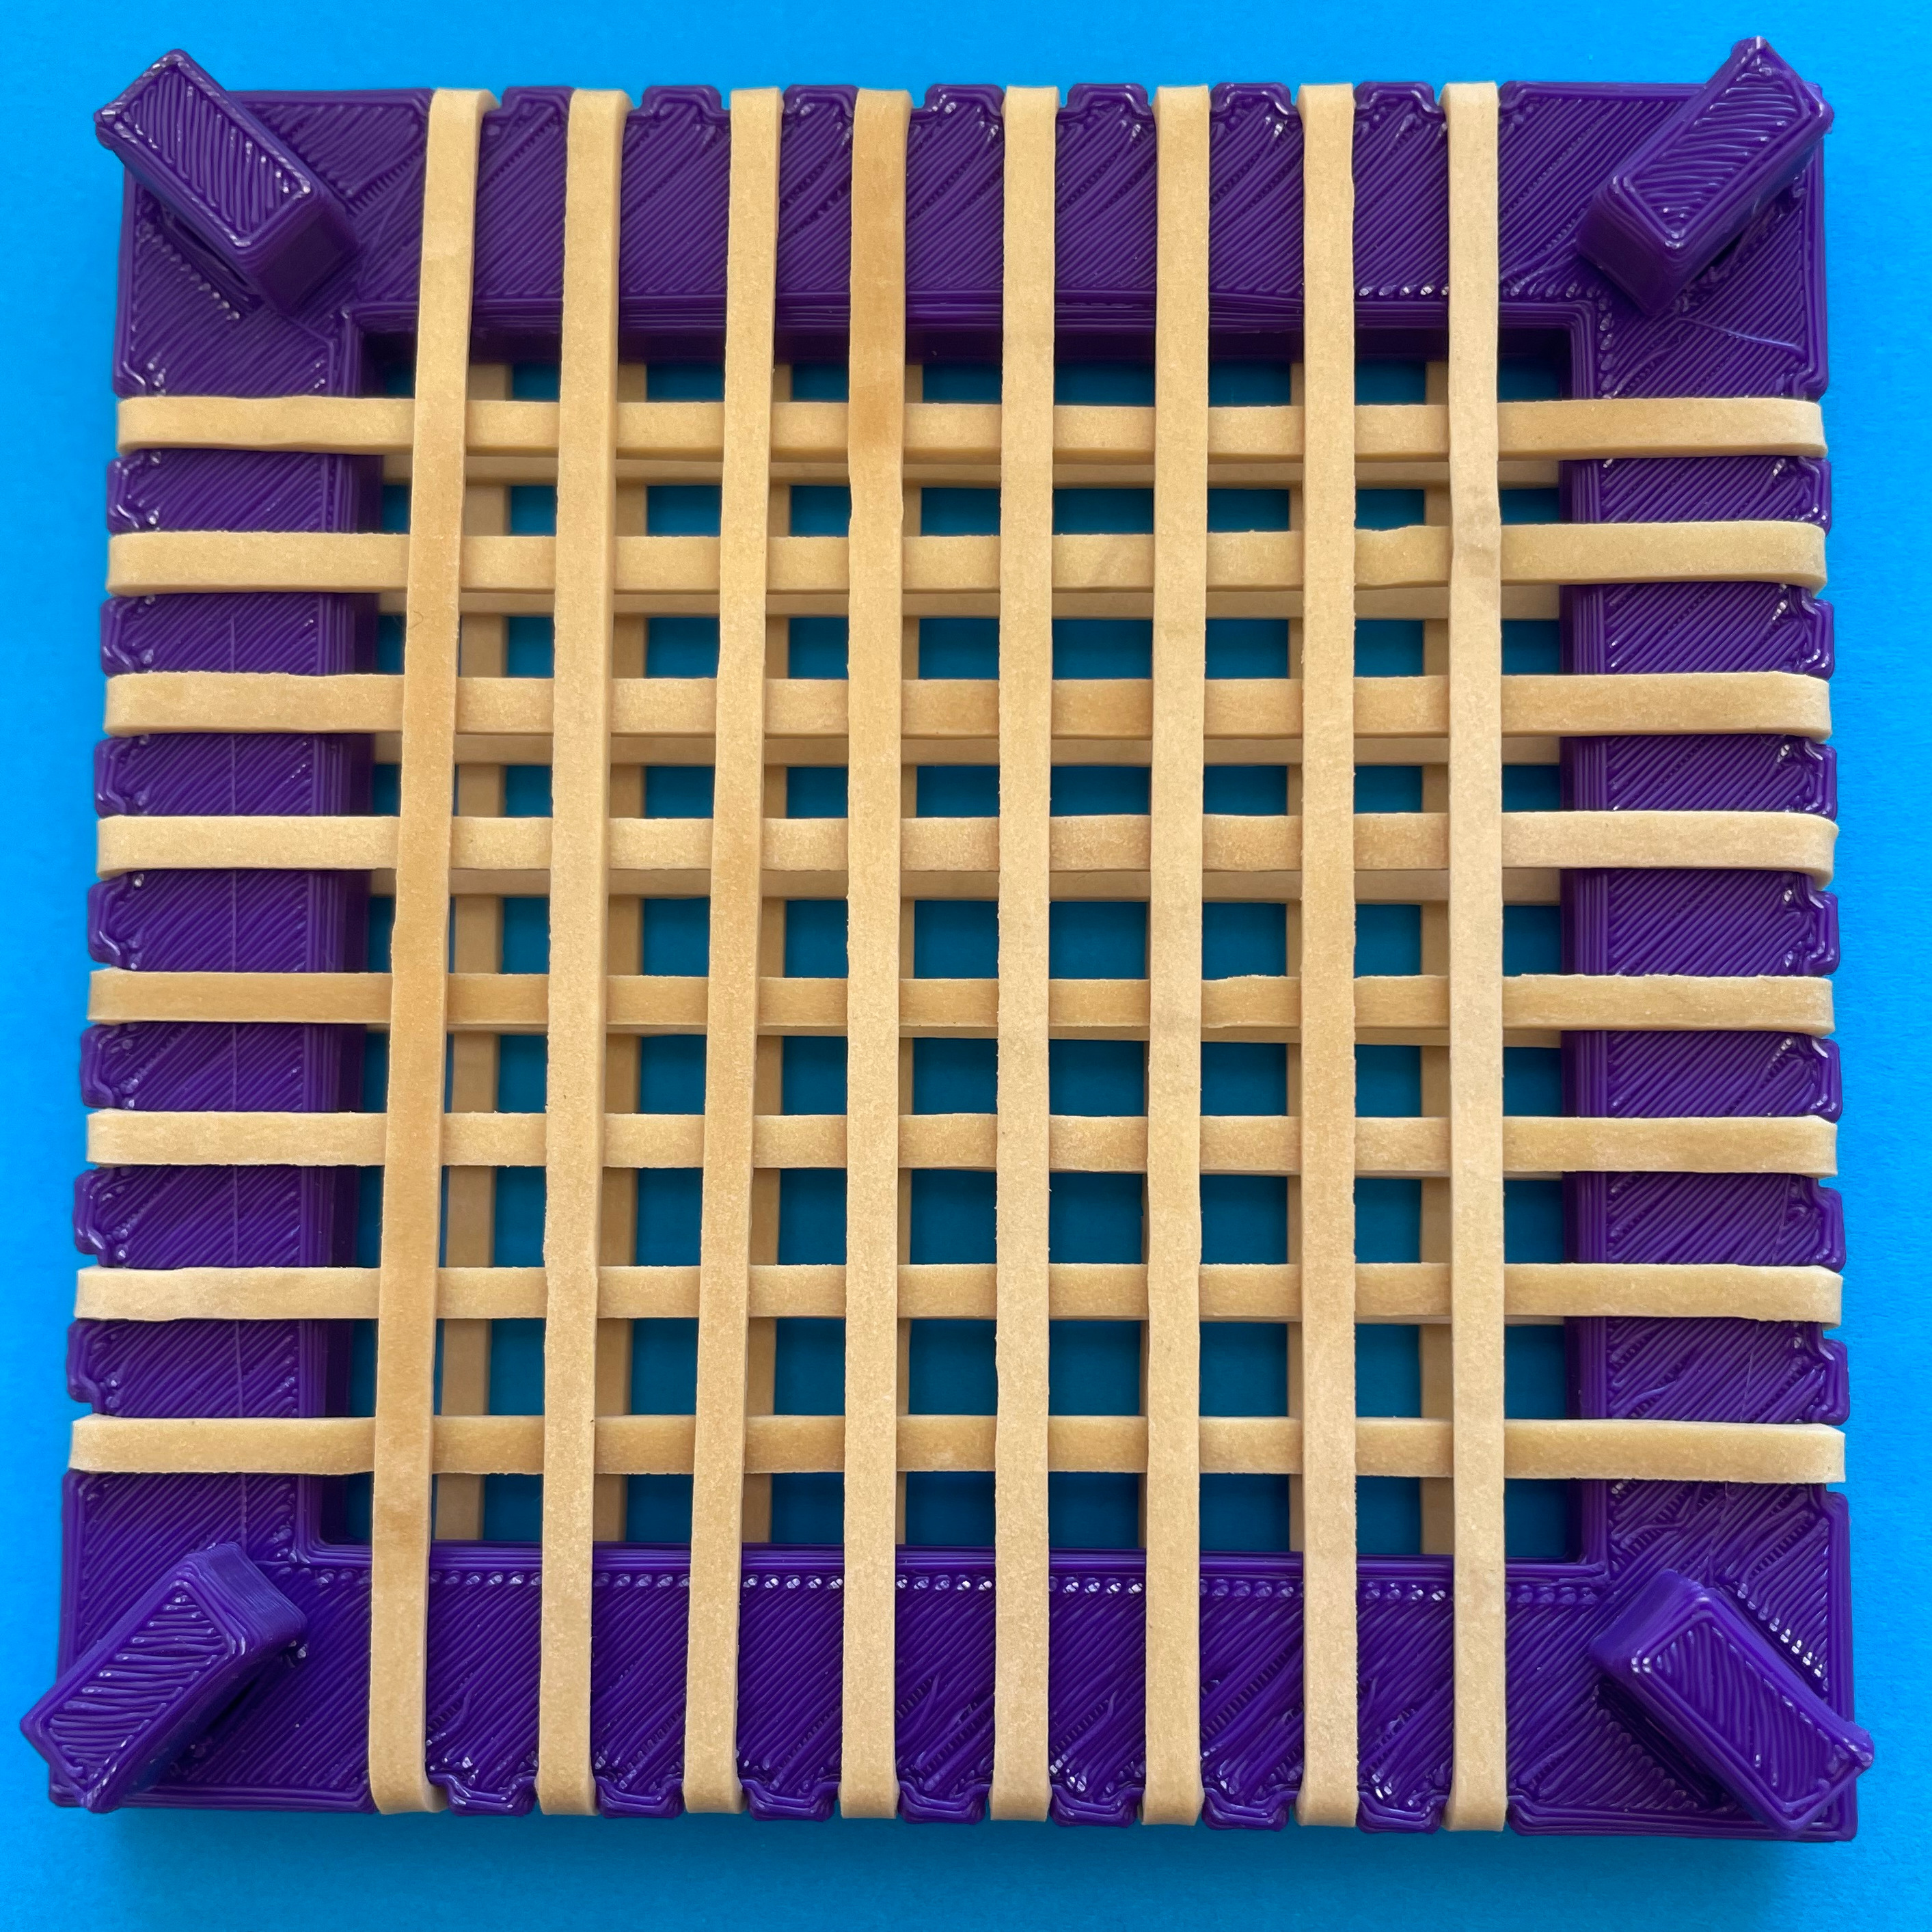
\includegraphics[width=\textwidth]{assembly_photo_4.jpg}
\caption{\raggedright \ Insert the feet into the}
diamond-shaped holes in the trampoline frame.
\end{subfigure}
\bigskip
\caption{Assembling the trampoline frame.}
\end{figure}
 
\newpage

\section*{Components}
\begin{multicols}{2}
\begin{itemize}[leftmargin=*]
%	\item 1 game box
	\item 1 trampoline
	\begin{itemize}[leftmargin=*]
		\item 1 trampoline frame
		\item 4 trampoline feet
		\item 16 rubber bands
	\end{itemize}
	\item 20 scoring tokens
	\item 12 twelve-sided dice
	\item 1 scoring tray
%	\item 1 money pack
	\item 1 game box
\end{itemize}
\end{multicols}
\section*{Assembly}
You will need to assemble your trampoline before you can play your first game. You do not need to disassemble your trampoline between games. 

\begin{enumerate}[leftmargin=*]
\item Punch the trampoline frame and the trampoline feet out of the acrylic slug. You can discard the unused portion of the acrylic slug.
\item Loop eight rubber bands around the trampoline frame. Each of these rubber bands should run parallel to the top/bottom sides of the trampoline frame and pass through one of the sets of grooves in the left/right sides of the trampoline.
\item Loop the remaining eight rubber bands around the trampoline~frame. Each of these rubber bands should run parallel to the left/right sides of the trampoline frame and pass through one of the sets of grooves in the top/bottom sides of the trampoline frame. 
\item Insert the trampoline feet into the diamond-shaped holes near the corners of the trampoline frame. You may want to glue the trampoline feet into the trampoline frame. If you do, be sure to use an adhesive that is appropriate for use with acrylic.
\end{enumerate}

\newpage

\begin{figure}
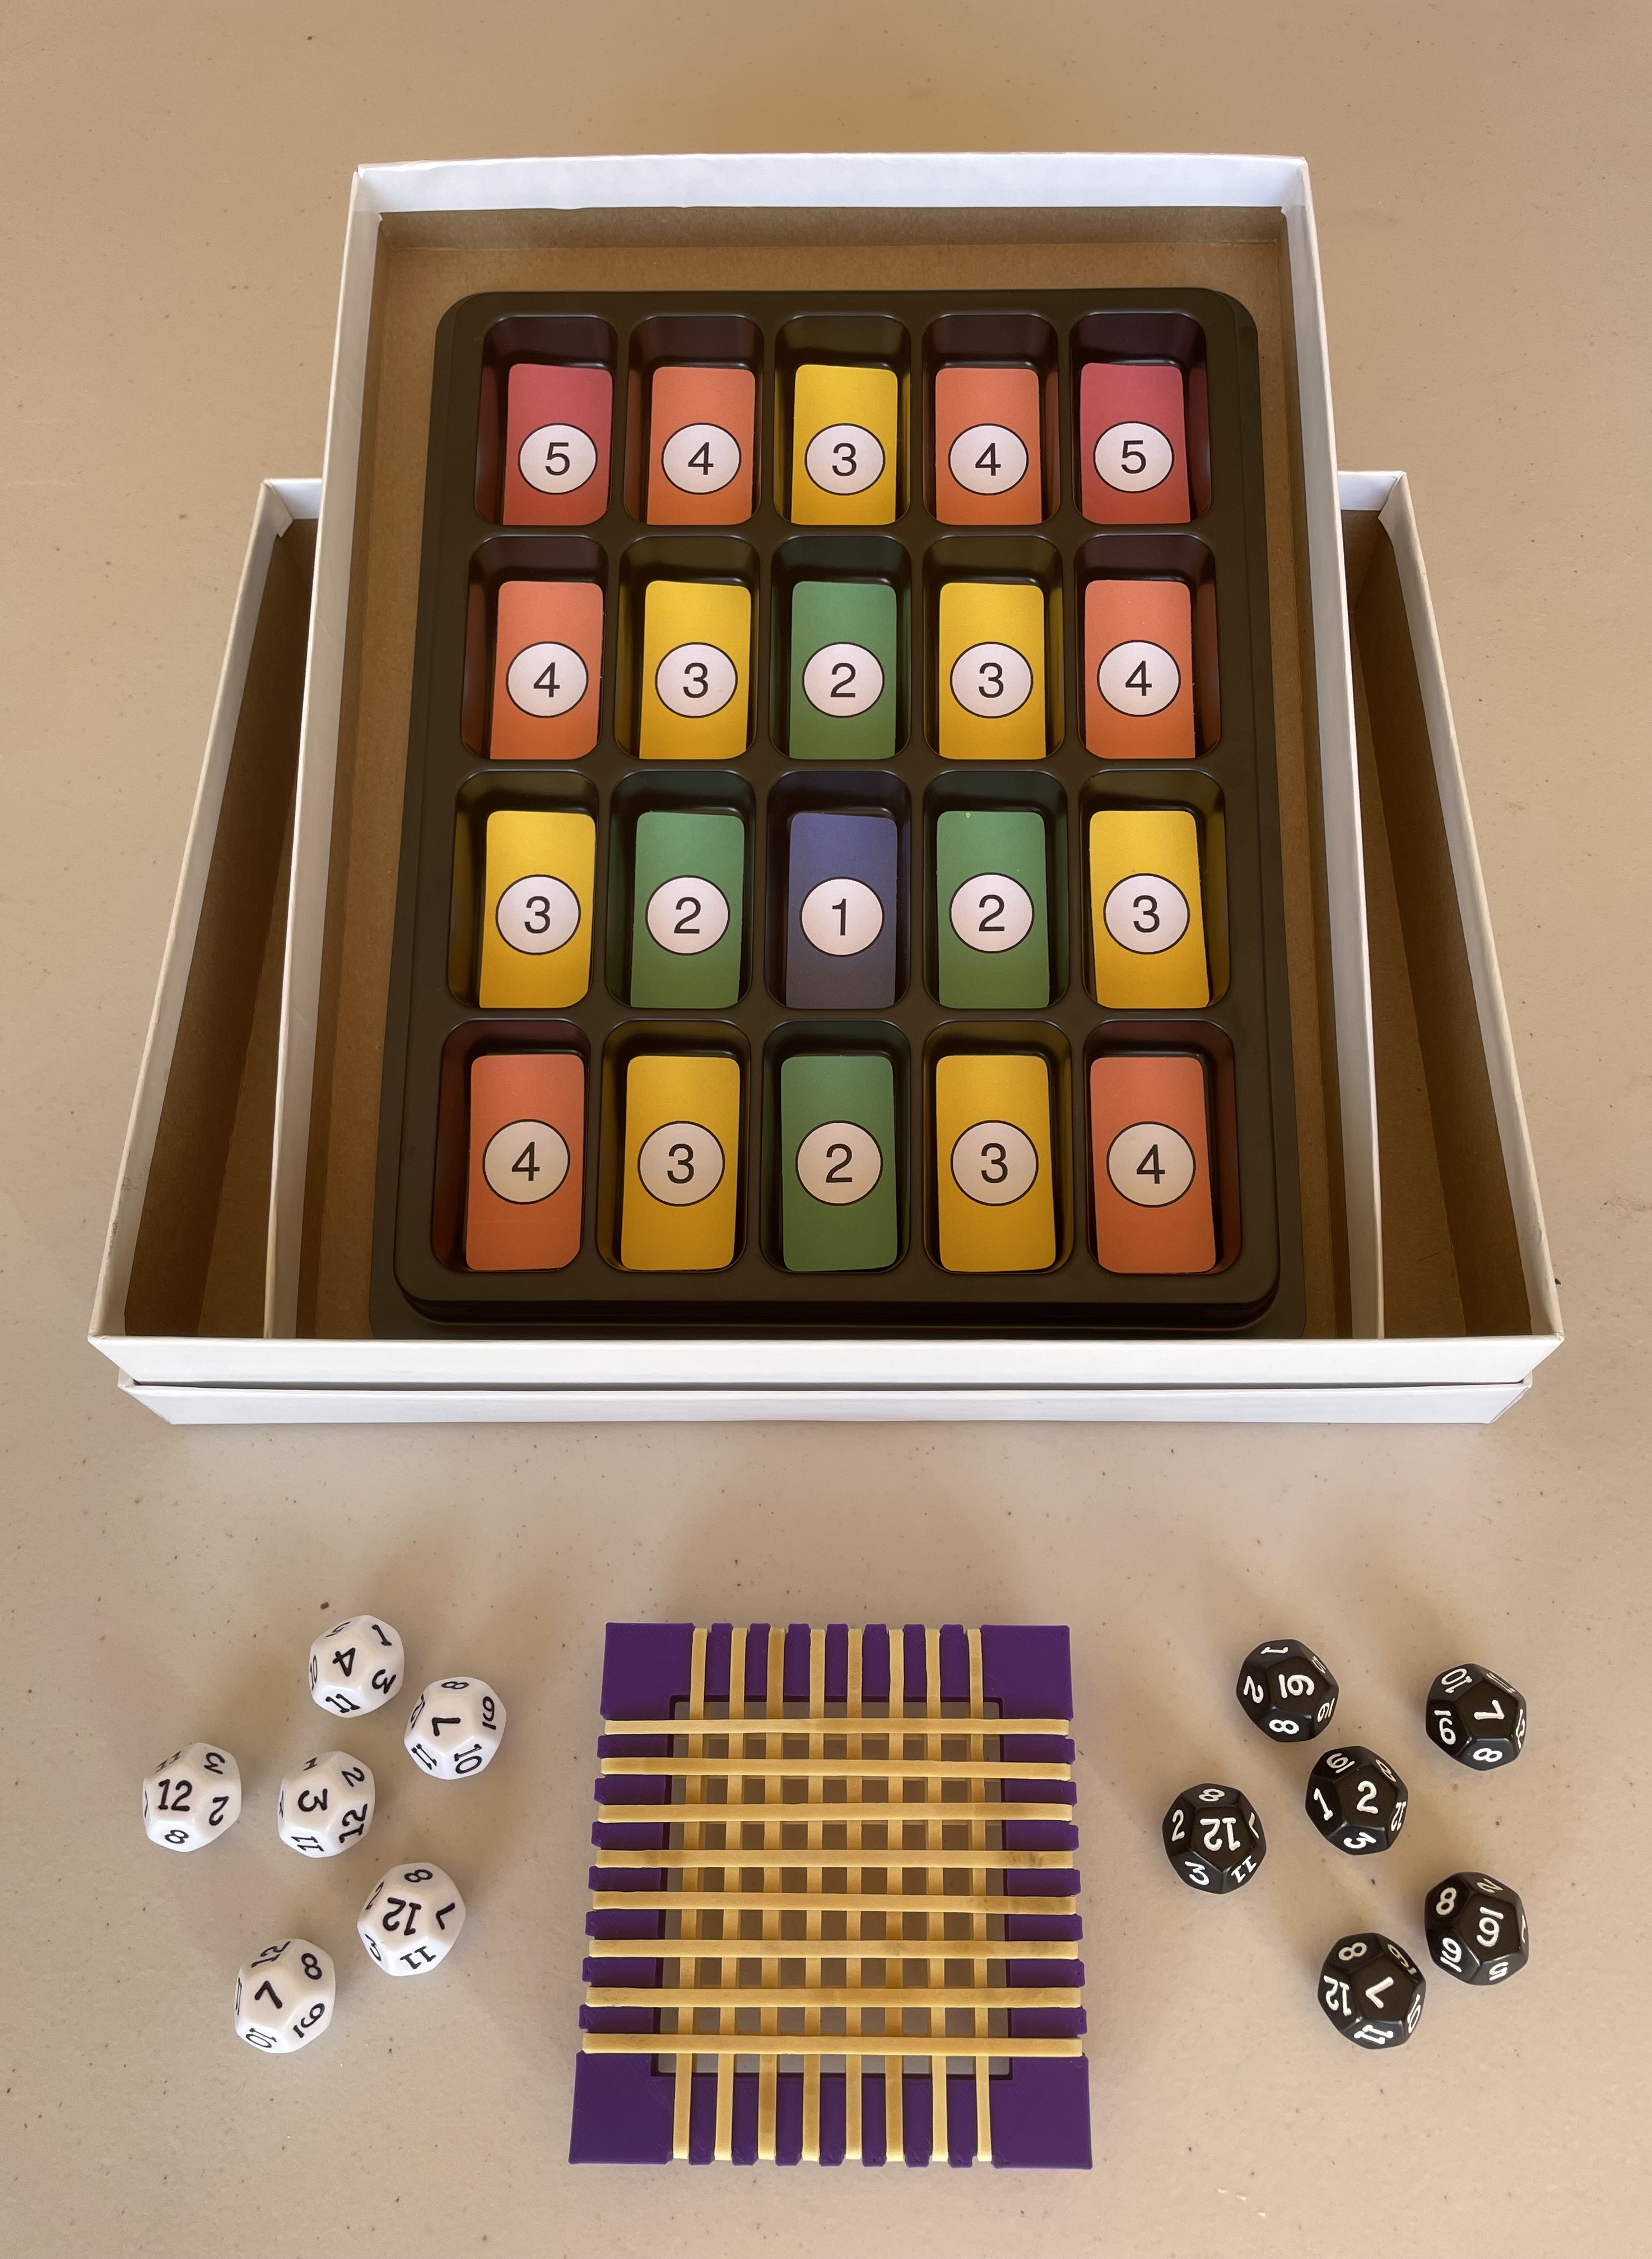
\includegraphics[width=\textwidth]{set_up_photo.jpg}
\bigskip
\caption{Setting up the game.}\label{figure:setup}
\end{figure}

\section*{Overview}
During the game, you will take turns trying to bounce dice off of the trampoline and into the scoring tray. You will score points based on where your dice land. After both players have thrown all six of their dice, the player with the highest total score wins the game.

\section*{Set Up}
\begin{enumerate}[leftmargin=*]
\item Sit at a table next to your opponent. You should both be sitting on the same side of the table.
\item Assemble the game board.
\begin{enumerate}[leftmargin=*]
\item Place the bottom of the game box in the middle of the table so that its interior is facing upwards. Orient it so that its long edge is facing you.
\item Place the top of the game box inside the bottom of the game box so that its interior is facing upwards. Orient it so that its short edge is facing you.
\item Place the scoring tray on the angled surface formed by the top of the game box so that the compartments are facing upwards.
\item Place the scoring tokens into the scoring tray as depicted in Figure \ref{figure:setup}.
\end{enumerate}

\item Place the trampoline on the table so that it is between you and the game board. 
%\item Place the money pack within easy reach of both players.
\item Randomly assign one player to be the first player. That player will use the black dice. The other player will use the white dice. Give each player all six dice of their dice. 
\end{enumerate}

\newpage
\section*{Gameplay}
On your turn you will do the following: 
\begin{enumerate}[leftmargin=*]
\item Reposition the trampoline. You may move the trampoline wherever you like provided that all four of the trampoline feet remain on the table.
\item Choose one of your dice to throw. You may throw each of your dice one time during the game.
\item Throw your die. It must bounce off of the trampoline. It must not touch the tabletop.
\item Score points based on where your die lands (see {\textcolor{blue}{\setmainfont{Century Gothic}\textbf{Scoring}}}). %Use bills from the money pack to track your score.
\item Clean up. If your die landed in one of the compartments of the scoring tray, leave it there. Otherwise, place it in the game box beneath the elevated edge of the scoring tray to help prevent any confusion about what dice remain in your supply.
\end{enumerate}

\section*{Scoring}\label{section:scoring}
You will score points based on where each of your dice lands after you throw them.
\begin{itemize}[leftmargin=*]
\item You score zero points if your die did not land in one of the compartments of the scoring tray or if it touched the tabletop after you threw it.
\item Otherwise, you score points equal to the number displayed on the scoring token in the compartment where your die landed times the number of dice in that compartment.

For example, the first die to land in a compartment with a ``3'' scoring token scores three points. The next die (of either color) to land in that compartment scores six points.
\end{itemize}

\begin{figure}
\raggedright
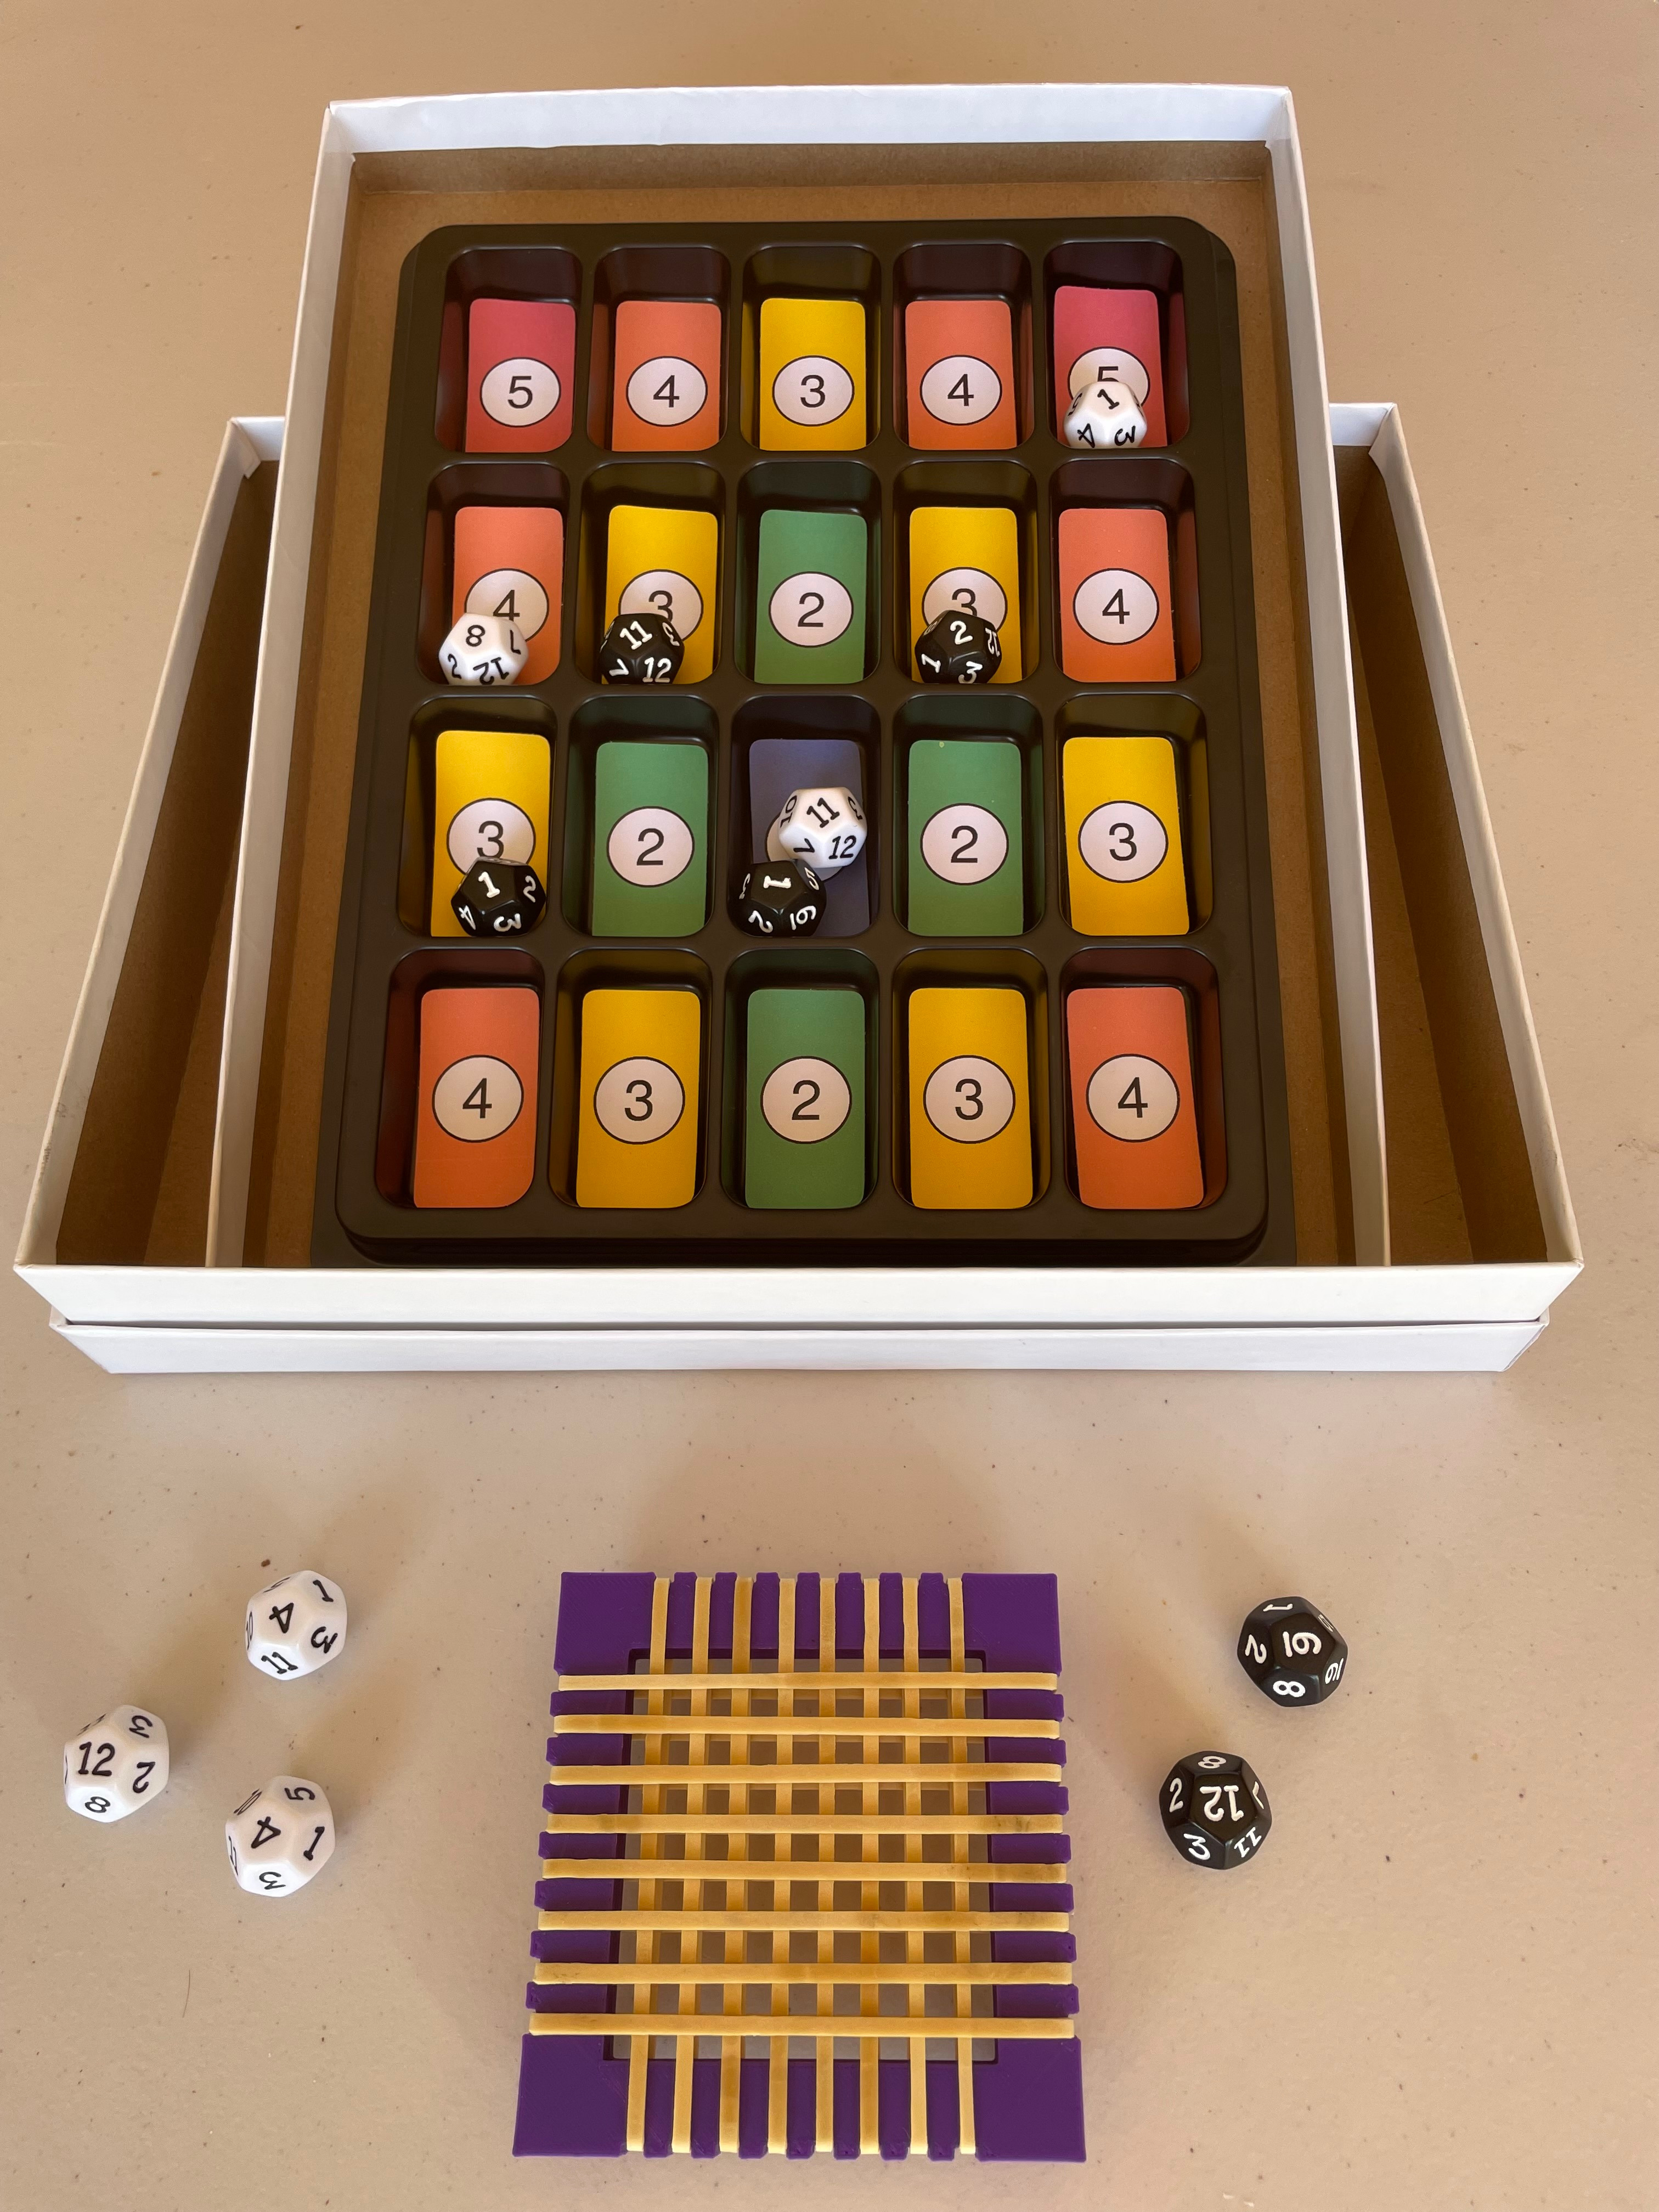
\includegraphics[width=\textwidth]{rebound_action_shot_3.jpg}
\bigskip
\caption{Scoring a mid-game position.}
\bigskip
\textbf{Example:} The first player has thrown four of their black dice and scored a total of $3+3+1+3 = 10$ points. The other player has thrown three of their white dice and scored a total of $4 + (2\times 1) + 5 = 11$ points.
\end{figure}

\newpage
\AddToShipoutPictureBG*{
\includegraphics[width=\paperwidth,height=\paperheight]{blue_page.jpg}}

\phantom{test}
\end{document}